
\documentclass[10pt,conference]{IEEEtran}

\ifCLASSINFOpdf
	\usepackage[pdftex]{graphicx}
	%\graphicspath{{./figs/}}
	\DeclareGraphicsExtensions{.pdf,.jpeg,.png}
\else
	\usepackage[dvips]{graphicx}
	%\graphicspath{{./figs/}}
	\DeclareGraphicsExtensions{.eps}
\fi

\usepackage[cmex10]{amsmath}
\usepackage[tight,footnotesize]{subfigure}
\usepackage{xcolor}
%\usepackage[lined,ruled]{algorithm2e}


\usepackage{algorithm}
\usepackage[noend]{algpseudocode}

\makeatletter
\def\BState{\State\hskip-\ALG@thistlm}
\makeatother


\usepackage[latin1]{inputenc}
\usepackage{tikz}
\usetikzlibrary{shapes}
\usetikzlibrary{arrows}

%\usepackage[]{algorithm2e}

\newtheorem{property}{Property}
\newtheorem{proposition}{Proposition}
\newtheorem{theorem}{Theorem}
\newtheorem{conjecture}{Conjecture}
\newtheorem{question}{Question}
\newtheorem{definition}{Definition}
\newtheorem{corollary}{Corollary}

\makeatletter
\pgfdeclareshape{datastore}{
\inheritsavedanchors[from=rectangle]
\inheritanchorborder[from=rectangle]
\inheritanchor[from=rectangle]{center}
\inheritanchor[from=rectangle]{base}
\inheritanchor[from=rectangle]{north}
\inheritanchor[from=rectangle]{north east}
\inheritanchor[from=rectangle]{east}
\inheritanchor[from=rectangle]{south east}
\inheritanchor[from=rectangle]{south}
\inheritanchor[from=rectangle]{south west}
\inheritanchor[from=rectangle]{west}
\inheritanchor[from=rectangle]{north west}
\backgroundpath{
    %  store lower right in xa/ya and upper right in xb/yb
\southwest \pgf@xa=\pgf@x \pgf@ya=\pgf@y
\northeast \pgf@xb=\pgf@x \pgf@yb=\pgf@y
\pgfpathmoveto{\pgfpoint{\pgf@xa}{\pgf@ya}}
\pgfpathlineto{\pgfpoint{\pgf@xb}{\pgf@ya}}
\pgfpathmoveto{\pgfpoint{\pgf@xa}{\pgf@yb}}
\pgfpathlineto{\pgfpoint{\pgf@xb}{\pgf@yb}}
 }
}
\makeatother

\newcommand{\riham}[1]{{\color{red}{#1}}}
\newcommand{\james}[1]{{\color{blue}{#1}}}


\begin{document}
\title{CS512 Course Project: Graph-based recommendation system for Yelp dataset challenge - Fall 2016}
\author{
\IEEEauthorblockN{Hanxiong Wang}
\IEEEauthorblockA{Rutgers University\\Netid:hw277\\
Email: hanxiong.wang@rutgers.edu
}

%\and
%\IEEEauthorblockN{Yingjiao Liang}
%\IEEEauthorblockA{Rutgers University\\Netid:yl977\\
	%Email: yl977@scarletmail.rutgers.edu}
%\and

%\IEEEauthorblockN{Dong Shi}
%\IEEEauthorblockA{Rutgers University\\Netid:ds1386\\
%Email: ds1386@scarletmail.rutgers.edu}

}

\maketitle
\begin{abstract}
\textnormal{
Recommendation system can be used in many commercial areas, e.g. food market, travel market and moive industry. In this project, a graph-based algorithm for a recommendation system is developed combining with collaborative filtering and item-based methond . We compute the accuracy and efficiency of the algorithm. The results shows that...
}
\end{abstract}
%\onecolumn \maketitle \normalsize \vfill

\IEEEpeerreviewmaketitle
%%%%%%%%%%%%%%%%%%%%%%%%%%%%%%%%%%%%%%%%%%%%%%%%%%%%%%%%%%%%%%%%%%%%%%%%%%%%%%%%%%%%%%%%%%%%%%%%%%%%%%%%%
\section{Project Description}\label{sec:1. Project Description}
%%%%%%%%%%%%%%%%%%%%%%%%%%%%%%%%%%%%%%%%%%%%%%%%%%%%%%%%%%%%%%%%%%%%%%%%%%%%%%%%%%%%%%%%%%%%%%%%%%%%%%%%%

%\textnormal{
%Insert your overall project description here. Specify the project type according to the posted sakai announcement.What is it that you are proposing?. Why is it useful?. Is it feasible to complete your project within the semester?.  Is it a novel idea?  What are the main stumbling blocks? What is the timeline for your project progress?. How are you planning to reach the major milestones?. 
%}

%The project has four stages: Gathering, Design, Infrastructure Implementation, and User Interface.

%\subsection{Stage1 - The Requirement Gathering Stage. } \label{sec:1	Requirement Gathering Stage. } 
%\input{Stage1.tex}
\subsection{Stage1 - The Requirement Gathering Stage. }\label{sec:1 Requirement Gathering Stage. }
%%%%%%%
%\textnormal{
%%%%%%
%} 

\begin{itemize} 


\item{
	The general system description: We develop a graph-based recommendation system combining both collaborative filtering and item-based method. The aim of the recommendation system is to provide users a most accurate recommendation list according to user habits. This system could be used in various business and commercial websites, e.g., Amazon, Yelp, IMDb and TripAdvisor, which includes almost all the daily area. Advantages and disadvantages of the algorithm for implementation will be shown. We utilize a free datasets including both user and business information from Yelp Dataset Challenge: https://www.yelp.com/dataset challenge.

} 


\item{	
	
The three types of users: 
people who seeks for recommendations in traveling, restaurant/food or hotel accommodation.
	
} 


\item{	

The user's interaction modes: the system uses a graphic user interface (GUI) as interaction mode with the user, where the user can input his/her information/preferences possibly through graph-based, discrete-feature terms or even simple personal identity. The system will output a set of nodes (i.e. suggested cities, restaurants or hotels, etc.) as graph or text format. 
	
}

\item{The real world scenarios: }
	\begin{itemize} 
	\item{Scenario 1 description: }
	A user of our recommendation system is concerned what to eat for dinner. He/She wants to pick some new restaurant that satisfies his/her taste best while maintaining a low spending according to the budget restraint. Our system will detect users that share similar tastes based on location, food style, and rating on restaurant that similar user has previously been to, and then recommend several restaurants to our user that he/she would potentially like to try, which also takes budget into consideration.
	\item{System Data Input for Scenario1: } 
	Spending, preferred cooking style, location, minimum overall rating
	\item{Input Data Types for Scenario1: }
	Nodes on the graph represent users. Edges indicate what restaurant those users have been to.  Weights of edges represent an overall measurement of how well a user likes a restaurant based on the input variables. 
	\item{System Data Output for Scenario1: }
	Restaurant recommended by our system.
	\item{Output Data Types for Scenario1: }
	Nodes which represent restaurant.  
	\item {Scenario 2 description: }
	A user of our system is in town on a business trip,and he only has limited time for lunch, and he wants to explore the best restaurant within a certain distance so that he can finish his lunch in time. And he does not care spending. Our system will finds out possible restaurants nearby, and recommend a list that most fit the users taste by searching restaurant raters with similar taste to our user.
	\item{System Data Input for Scenario2: } 
	Preferred cooking style, location, maximum distance, minimum overall rating.
	\item{Input Data Types for Scenario2: }
	Nodes on the graph represent different users. Edges indicate what restaurant those users have been to.  Weights of edges represent an overall measurement of how well a user likes a restaurant based on the input variables. 
	\item{System Data Output for Scenario2: }
	Restaurants recommendation by our system.
	\item{Output Data Types for Scenario2: }
	A list of nodes which represent restaurant.  
	\end{itemize}

\item{Project Time line.}
	\begin{itemize}
	\item{Stage 1: Oct. 14 to Oct. 25, 2016 } 
	 We will be working on the requirement gathering stage, which includes topic and data selection, model selection, input and output set up, as well as labor division.
	 \item{Stage 2: Oct. 26 to Nov. 10, 2016 }
	 Will be working on the deign of algorithm stage. Transformation on the project requirement into a system flow diagram will be done. We will carry out high level pseudo code of the overall system operation, and give a statement on run time and space complexity. 	
	 \item{Stage 3: Nov.11 to Nov.24, 2016}
	 Will be working on the implementation stage. Programming language and environment will be settled down. Code, demo and sampling of  finding will be done by Nov.25
	 \item{Stage 4: Nov.25 to Dec.9, 2016}
	 Will be working on the implementation of user interface. Our system will output proper recommendation based on the input.
	 \item{Final stage: Dec.9-Dec.16, 2016}
	 Final report composition and presentation materials will be done by the due date.
	\end{itemize}
	
%\item{Division of Labor.}
%	 \begin{itemize}
	% \item{Dong Shi}
	 %Report generation, design of the graph-drawing based algorithm
	 %\item{Yingjiao Liang}
	 %Report generation, design of the graph-drawing based algorithm
	 %\item{Hanxiong Wang}
	 %Report generation, design of graph-drawing based algorithm, UI design, working code
	 %\end{itemize}
 

\end{itemize}


\subsection{Stage2 - The Design Stage. }\label{sec: 2:The Design Stage.}
%%%%%%%%%%%%%%%%%%%%%%%%%%%%%%%%%%%%%%%%%%%%%%%%%%%%%%%%%%%%%%%%%%%%%%%%%%%%%%%%%%%%%%%%%%%%%%%%%%%%%%%%%%
%\begin{itemize} 
%\item{ }
%A brief textual description of the overall flow diagram (along with its functional operation in the different user scenarios described in the first stage of the project).
%\item{ }
%A specification of each algorithm and associated data structures together with its entities, attributes, and operations ( include an English description of how they relate to your user scenario(s)).

%\end{itemize}

\begin{itemize} 
\item{  Short Textual Project Description. }

Here, for conveniently understanding and evaluating our project, a recommendation system for users who are in demand of public services, like restaurants, pet shops, or grocery stores, is illustrated as an example. From our Yelp Dataset, as mentioned above, we extract three key factors, including user's ratings, the category of a business unit and its attributes (i.e. prices for different foods, alcohol provider or not, payment ways, Wi-Fi service, good for group food or not, good for kids or not, easy-appointment access, reservation time and wheelchair, etc.). The relative information between these entities (users and business unit) shows as graph edge weights in our algorithm, and will be calculated using users' ratings. When executing our recommendation system, an optimal recommendation list will be generated based on built-in grading function; and the recommendation list is composed of a set of users and business unit with some specific relationship. For examples, a list of restaurants are rated about the same within a certain set of users.\\


Flow diagram textual description:\\


1. Obtain raw dataset and collect the clean data satisfying the requirement for the further analysis using the procedure ``BUILD\_GRAP\_LIST", where the user, business units (business company) information and corresponding review (e.g. restaurant ratings) are collected and finally form an adjacent list for these information.

2. Build up the objective graph using three procedures: BUILD\_FIRST\_LAYER, BUILD\_SECOND\_LAYER and BUILD\_THIRD\_LAYER. Inside the objective graph, the edges weights between nodes in different definition layers (users and business units) are generated based on our specifically-designed algorithms. collaborative filtering; content based.

3. Generate a recommendation list with the procedure ``FORM\_REC\_LIST" with providing an accuracy/quality rate from the procedure ``EVALUATE\_ACCURACY".

4. Evaluate different recommendation lists by modifying and improving the algorithm input parameters with corresponding accuracy/quality rates by repeating Step 1to 3.

5. Select the best recommendation list with the optimal accuracy/quality rate.\\

In our algorithm, the space complexity is individual\_node\_unit * \textit{O}(\textit{N} = numbers of users and business units). Because the multiple pointers exist (i.e. a user can rate a lot of business units), individual\_node\_unit can be considered to use two ways: i) an adjacent list to preserve these points (PROS: minimize the space complexity; CONS: increase the algorithm complexity when building up the objective graph); i) an adjacent matrix (PROS: easy to access and build up an objective; CONS: have huge waste in space if the maximum rating number is very high and few users have provided multiple rating in different business units). We need to build up the objective graph and search the entire graph, based on different implementation methods, the optimal time complexity in our recommendation system is \textit{O}(\textit{E}*log(\textit{N})) $ \approx $ \textit{O}(\textit{N}*log(\textit{N}) (if multiple ratings are few), \textit{E} is the total edge.\\

\item{ Flow Diagram. }
\begin{figure}[h] \label{fig:flowDiag}
\begin{center}
    {\scalebox{0.3}{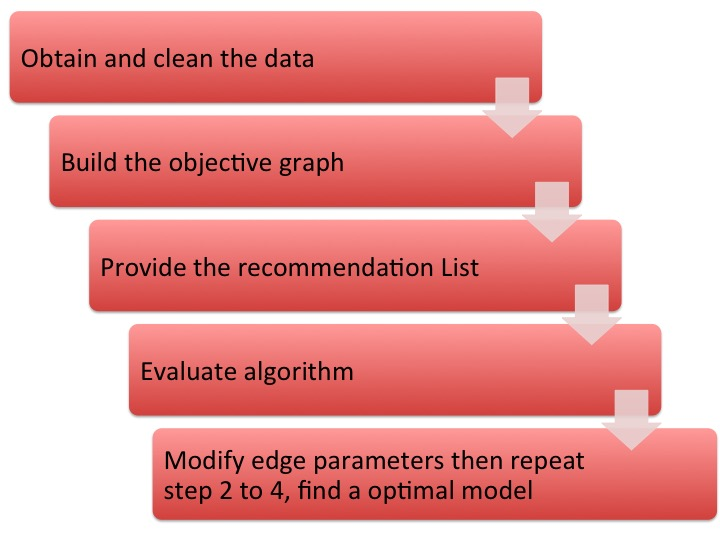
\includegraphics{FlowDiagram.jpg}}}
 \caption{Flow Diagram}
\end{center}
\end{figure}

\item{ High Level Pseudo Code System Description. }
\begin{algorithm}
\caption{Graph-based recommendation system}\label{algo-pseudo}
\begin{algorithmic}
\State Clean and import the data
%\State Partition dataset by user\_info, business\_info and view\_info, build the whole adjacent list of the graph by the clean dataset
\Procedure {Build\_Grap\_List}{}
    \State $\textit{user\_info} \gets \text{input user\_info}$
    \State $\textit{business\_info} \gets \text{input business\_info}$
    \State $\textit{review\_info} \gets \text{input review\_info}$
    \State $\textit{G\_list} \gets \text{build a adjacent graph list by the above dataset}$
\EndProcedure

\Statex

\State Build the objective graph
%\State Build the objective recommendation graph layer by layer (layer 0 is the objective node user A)

\Procedure{Build\_First\_Layer}{user node A, G\_list}
\State $\textit{find(first\_ln)} \gets \text{All nodes link to node A}$
    \ForAll {$node \in first\_ln$} 
          \State $node\_edge = RStar$ %\Comment {get edge from node A}
    \EndFor
\EndProcedure

\Procedure{Build\_second\_Layer}{\textit{first\_ln, G\_list}}
\State $\textit{find(second\_ln)} \gets \text{All nodes link to the first layer}$
    \ForAll {$node \in second\_ln$} 
          \State $node\_edge = RStar + RAve()$ %\Comment {get edge from nodes in first layer}
    \EndFor
\EndProcedure

\Procedure{Build\_third\_Layer}{\textit{first\_ln},\textit{second\_ln},G\_list}
\State $\textit{find(third\_ln)} \gets \text{All nodes link to nodes in second layer}$
    \ForAll {$node \in third\_ln$}
         \If {$node.cate \in set(first\_ln.cate)$}
                \State \textit{Aux(cate,attr) = Aux1(cate)+Aux(attr)}
         \Else
                \State \textit{Aux(cate,attr) = 0}
         \EndIf
    \EndFor                  
    \ForAll {$node \in third\_ln$} 
          \State $node\_edge = RStar + RAve()+ Aux(cate,attr)$ %\Comment {get edge from nodes in second layer}
    \EndFor
\EndProcedure

\Statex
\State Compute the longest path to each leaves and give the recommendation list

\Procedure {Form\_Rec\_List}{user node A, first\_ln, second\_ln, third\_ln}
    \State Rec\_List =\{\}
    \ForAll {$node \in third\_ln$}
         \State $node.lp() \gets \text{compute the longest path from node A} \hfill \break
         \text{\ \ \ \ \ \ \ \ \ \ \ \ \ \ \ \  \ \ \ \  \ \ \ \ by node.lp}$
    \EndFor
    Raw\_Rec\_List = sort(third\_ln) 
   \ForAll {$element \in Raw\_Rec\_List$}
         \If {$element \in first\_ln$}
                 \State do nothing
         \Else
                 \State Rec\_List.add(element)
         \EndIf
   \EndFor
\Return Rec\_List
\EndProcedure


\Statex
\State Provide the Accuracy Rate

\Procedure{Evaluate\_Accuracy}{}
    count = 0
    \For {$i \leftarrow 1 {\; \rm to\;} length(first\_ln)$}
            \If {$Raw\_Rec\_List[i] \in first\_ln$}
                     count +=1
            \EndIf
    \EndFor
\Return   Acc\_rate = count / length(first\_ln)        
\EndProcedure
\end{algorithmic}
\end{algorithm}

\item{Algorithms and Data Structures. }

Our algorithm design bases on such a basic idea: users who have similar taste in business units tend to review a specific business units with close score. Such a set of users should be a potential consumer group for some business units in a particular category. For example, finding out the people who love French cuisine is very meaningful if we can also recommend some good French restaurant to them. Thus, the first thing we do here is to correlate the similar patterns of users' rating from different business units; then we can recommend the favorite business units of a user to other users who have similar taste. 

The detailed contents and data structures of our algorithm pipeline are shown in ``Algorithm 1". In the part I - ``Clean and import the data", the raw data are provided and generated the specific data structure recording the ratings of each user for different restaurants: an adjacent list or an adjacent matrix for each user. In the part II - ``Build the objective graph", the users' rating data are built up as an objective graph data structure with specifically-designed edge weights by connecting users and business units with similar ratings, etc. In the part III - ``Compute the longest path to each leaves and give the recommendation list", we obtain list output using some algorithm similar to finding out the longest path in the directed acyclic graph (DAG). In the part IV - ``Provide the Accuracy Rate", a double floating value is provided by in order accessing each unit of the recommendation list from the part III.

\begin{figure}[h] \label{fig:representation_alg_1}
	\begin{center}
		\advance\rightskip-1cm
		{\scalebox{0.3}{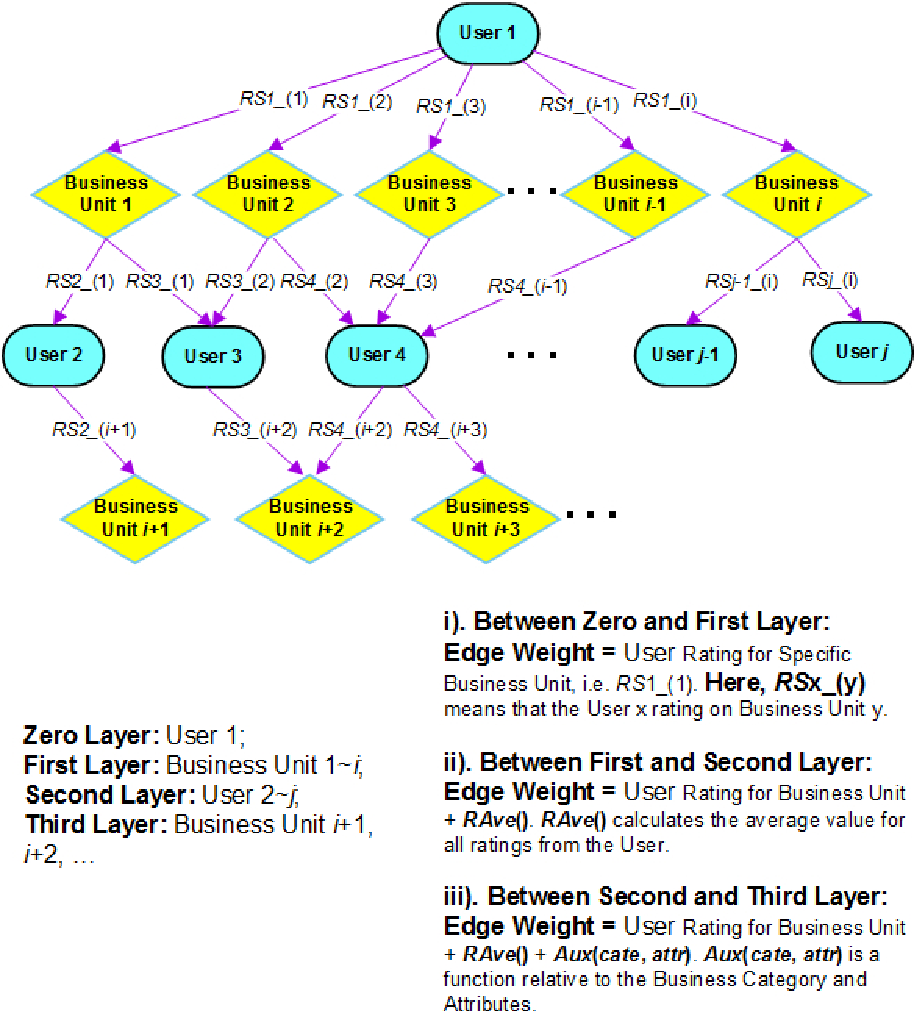
\includegraphics[width=300mm]{representation_alg_1.pdf}}}
		\caption{The objective graph representation in Algorithm 1}
	\end{center}
\end{figure}

\end{itemize}

\begin{itemize} 
\item{  Flow Diagram Major Constraints.}
\begin{itemize} 
\item{ Integrity Constraint. }
\\1. The input user need to have sufficient  reviews on record. Our recommendation system provides recommendation list by finding similar users based on input user's reviews. And it does so by comparing the reviews on business units that serve same purpose. The more reviews the input user has, the more accurate of measurement we have on its taste, and therefore, the better the recommendation can be.
\end{itemize}
%\begin{itemize} 
%Please repeat the pattern for each integrity constraint.
\end{itemize}


\subsection{Stage3 - The Implementation Stage. }\label{sec: 3 The Implementation Stage.}
%%%%%%%%%%%%%%%%%%%%%%%%%%%%%%%%%%%%%%%%%%%%%%%%%%%%%%%%%%%%%%%%%%%%%%%%%%%%%%%%%%%%%%%%%
%Specify the language and programming environment you used for your implementation.
%Building the corresponding relational tables, according to the proposed ER model described in the previous phase %enforcing the different integrity constraints.  
%The deliverables for this stage include the following items:
\begin{itemize} 
\item{Sample small data snippet}
%The SQL tables that represent the ER project model, along with at least 3-5 rows of concrete data per table.

Our data sets are composed of three classes, which include review data, user data, and business data. As we have mentioned in the context above, our recommendation system focuses on Pennsylvania centered business. Eventually, we have 32134 as total number of users, 111542 of reviews, and 4086 of business units. The figure below displays an original sample data structure in each of the classes.

\begin{figure}[h] 
	%\begin{center}
		\advance\rightskip-1cm
		{\scalebox{0.3}{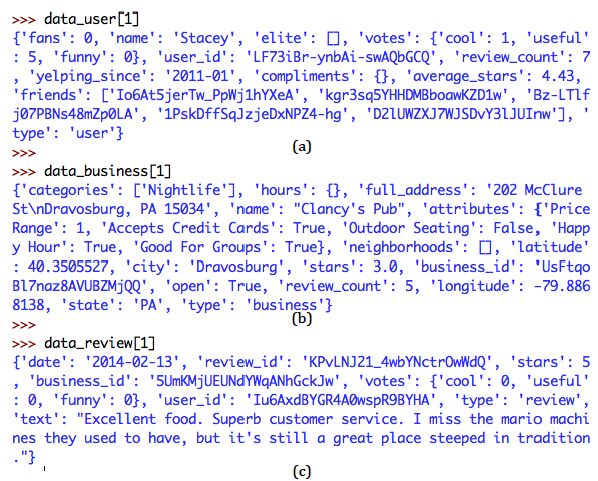
\includegraphics[width=300mm]{sample_data.png}}}
		\caption{Sample data: (a). User Data; (b). Business Data; (c).Review Data}\label{fig:Sample_Data}
	%\end{center}
\end{figure}

\par
We consider a variable significant if it can directly reflex or indirectly help to interpret a user's preference on business units. All the significant variables are then taken into consideration in the recommendation process, with more or less weight. 

For user data, average stars is the average review (level from 0 to 5) a user gave. User id is a unique id code assigned to each user. It is a key variable that relates the three classes of information. And review count, as the total number of review a user has given, will also be used, particularly in the evaluation step. 

For review data, stars indicate how much the reviewer liked this business unit. As star increases, the reviewer likes more. Business id represent each business unit. Finally, user id in review data indicates from who this review was given. 

As for the business data, categories and attributes will be used as characteristic description of a business units through our recommendation system. Business id is a unique code that represents a business store.

\item{Sample small output}
%The normalization steps for each table, along with explanations/justifications of each normalization step.

Given an eligible input user number, the recommendation system generates a recommendation list composed of all business units that has connection to the input user. Each element in the recommendation list has a total score measuring how similar this store is to something the user liked in the past.  Our system chooses business units with greatest score by determining the longest path from the root  node to each third layer nodes. Then it outputs the top ten on which input user has not reviewed before. The result will be an optimal solution based on our item plus user based collaborative filtering algorithm. Below is an example of data output for user 74. 

\begin{figure}[h] 
	\begin{center}
		\advance\rightskip-1cm
		{\scalebox{0.2}{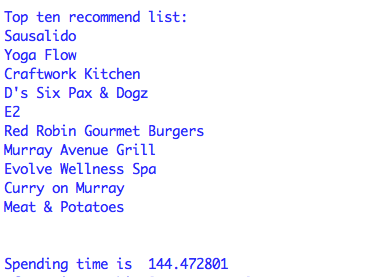
\includegraphics[width=300mm]{sample_output.png}}}
		\caption{Recommendation list for user 74  }\label{fig:Sample_Output}
 \label{fig:top10RecList}
	\end{center}
\end{figure}

\par
As a result, our system is built with relatively hight accuracy and stability. We will show this in following section.
 
\item{Working code}

The code package, as a compressed file with the zip format, is attached in the report. Package includes two zip file named as: maincode.zip and data\_preparation.zip.

\item{Representative of Sample Dataset and Data Size Analysis}
\par
Due to the relatively huge volume of the ``yelp academic dataset", it requires a long processing time for a normal desktop/laptop to execute the data mining task through the whole data set. Thus, only the data from the state of Pennsylvania (labeled as PA in the dataset) are extracted in execution as a sample/demo of our recommendation system. Based the design, our system mainly composes of two sub-procedures: i). generating of clean dataset with specific data structure; ii). Simulating a recommendation list of business units with a given user ID. Here, we provide a space analysis and a demo in the Non-graphical interface.

\par
There are three subsets in the PA data related to business dataset, users dataset and review dataset preserved as the specifically compressed format with sizes of about 5 MB, 19 MB and 111 MB, respectively. All of them are loaded in the RAM. In order to conveniently investigate the required RAM space for the objects during the execution, we utilize the functions in the packages of ``cython" and ``meliae" of Python. These data are separately loaded in the RAM and checked for the required space. The results are shown in Fig. \ref{fig:RAM}. We can see that review dataset requires the maximum RAM space. It is reasonable because the reviews might include some statements with connecting both users and business units. As seen, most of the space are dominated by the unicode strings data (52\%, 47\% and 64\% for the business, user and review dataset, respectively). The total RAM is 555 MB when loading all dataset into RAM with 49 types of variables, which is shown in Fig. \ref{fig:RAM_total}.

\begin{figure}[h] 
	\begin{center}
		\advance\rightskip-1cm
		{\scalebox{0.28}{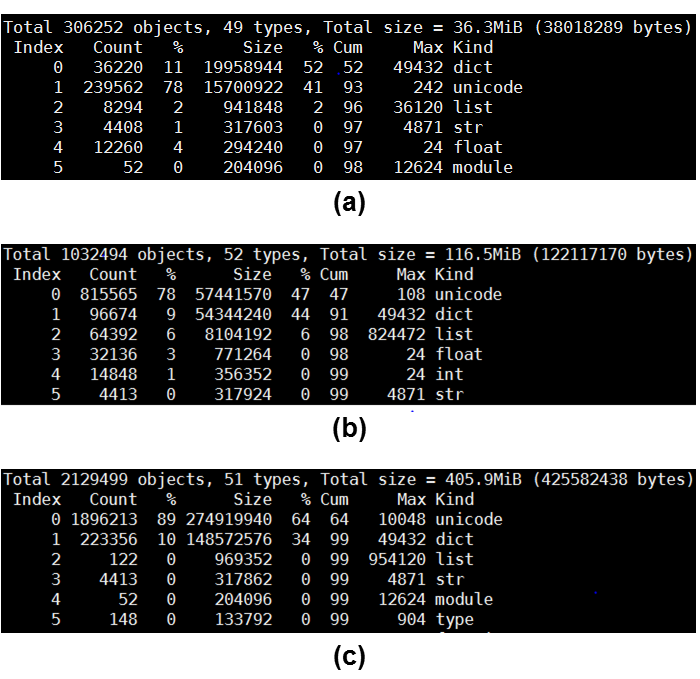
\includegraphics[width=300mm]{RAM.png}}}
		\caption{The require RAM analysis for the input dataset: (a). only business dataset loaded; (b). only user dataset loaded; (c). only review dataset loaded, respectively. The analysis results are from the package of "meliae" in Python.}\label{fig:RAM}
	\end{center}
\end{figure}

\begin{figure}[h] 
	\begin{center}
		\advance\rightskip-1cm
		{\scalebox{0.3}{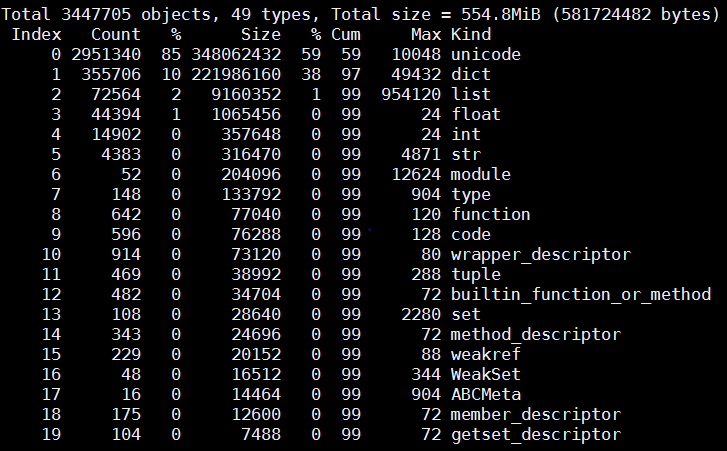
\includegraphics[width=300mm]{RAM_total.png}}}
		\caption{The require RAM analysis for loading the whole representative sample dataset collected from the package of "meliae" in Python.}\label{fig:RAM_total}
	\end{center}
\end{figure}

\item{Sample findings and Demo Result}

As pointed out in the ``Integrity Constraint" subsection, the performance of recommendation system depends on the dataset. In fact, this is one of the basic problem in any task relative to data mining system: valid data is often small. In our system, we can roughly estimate the size of valid data using two rat parameters: the reviews per business unit and the reviews per user. To some extent, we will hope these two ratios are high, which means that there are relationships between the observed users and business units. In our sample data, the reviews per business unit and the reviews per user are 27 and 3. The reviews per business can provides a reference what is a roughly average depth of a recommend graph/tree in our system; in the other hand, the reviews per user can provides a reference about how many new users involved in the next level. To analyze both them in whole dataset might be an extremely complicated task considering that each user has its specific recommendation graph network. Thus, to be simple, we only analyze the distribution of review count per user as shown in Fig. \ref{fig:review_count_per_user}. The distribution is a smooth decreasing curve with the highest point in 1. This means that about 5000 of 32134 users have only a review. As we can see, the curve decrease very fast and the count of users is about 500 when user's review number is at 15. This indicates that only part of users kept writing down their reviews for different business units; this also means that these users have more relationships with others. Our system can provide better recommendation for these users by constructing their graph network with more features. 

\begin{figure}[h] 
	\begin{center}
		\advance\rightskip-1cm
		{\scalebox{0.28}{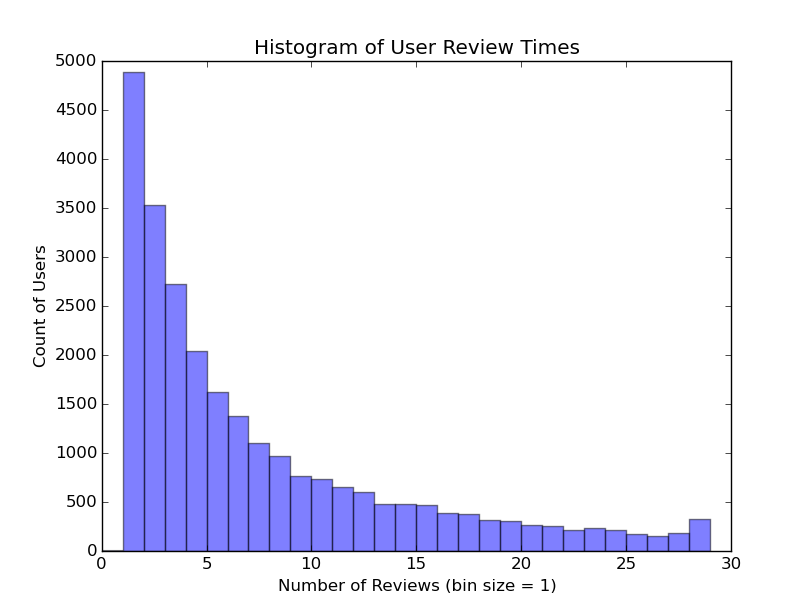
\includegraphics[width=300mm]{review_count_per_user.png}}}
		\caption{Histogram of the reviews for different business units.}\label{fig:review_count_per_user}
	\end{center}
\end{figure}

A demo in the Non-graphical interface is also displayed in Fig. \ref{fig:demo_pipeline}. Here, our system simply accepts the user ID (an integer number) as the input rather than a users' name. Then, a network graph/tree is constructed for the specific input. By following this, our system will extract the existing attributes from the network to look for favorite recommendation with the setting parameters. Finally, a recommendation list including various business units is displayed. This list indicates this user might be interested at looking for the potential consumption from these business units. The performance and execution of our systems strongly depends on the number of existing relationships between the input user and other users. More relationship will induce better performance with fast increasing running time requirement, mainly from the construction of a relationship network.\\ 

\begin{figure}[h] 
	\begin{center}
		\advance\rightskip-1cm
		{\scalebox{0.35}{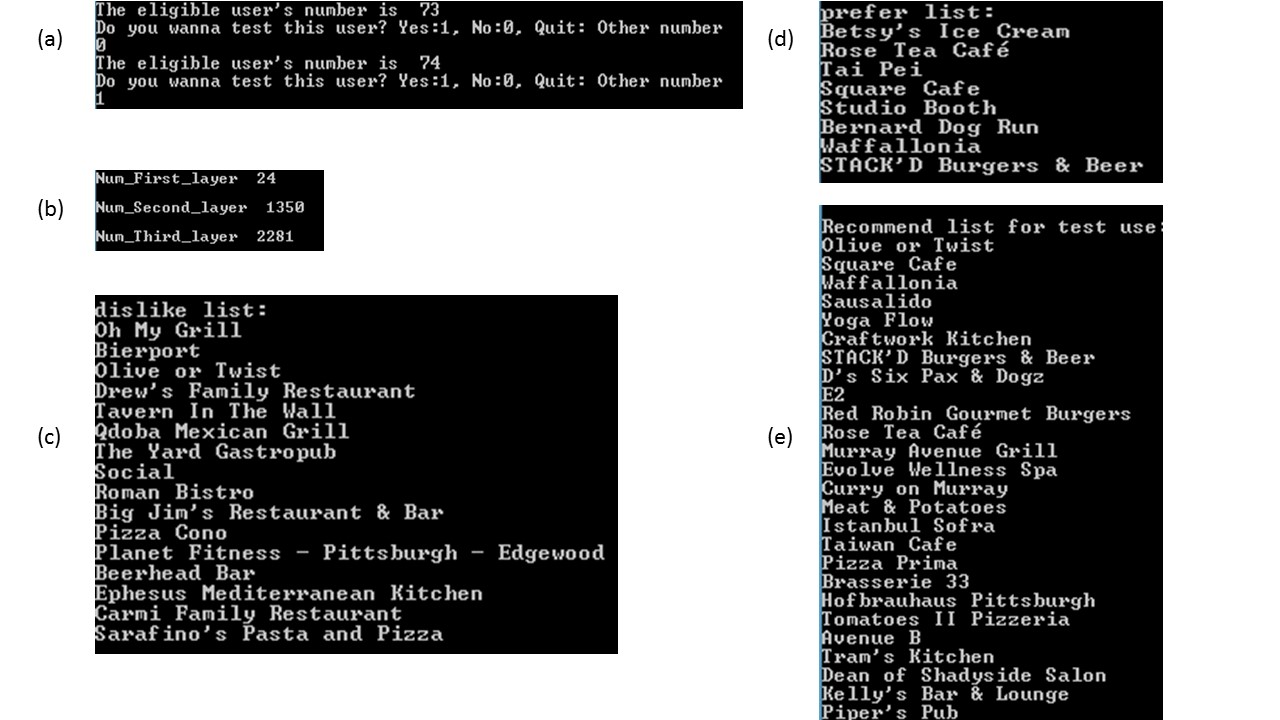
\includegraphics[width=300mm]{demo_pipeline.jpg}}}
		\caption{A demo in the Non-graphical interface: (a) In cmd, using commend "python RecomSys.py" to run the system. A user ID is provided as input. You can execute our recommendation by clicking 1 or skip by clicking 0. Clicking 0 will generate another user ID. Just click any key rather than 0 or 1 to turn off the execution.  (b) The number of nodes (Business Units or Users) in the first three layers are displayed. The first and third layer includes the business units as nodes and the second layer are the users as nodes, who have reviewed the business units in the first layer. (c) A disliked business unit list according to root user in the first layer is also provided. (d) A preferred business unit list according to root user in the first layer is represented. (e) Part of the recommendation list for the test use.(Not the final recommendation list, need remove the business unit that user has already reviewed.)}\label{fig:demo_pipeline}
	\end{center}
\end{figure}

\item{Evaluation on the Algorithm Performance}
\par
It is hard to know if a user is satisfied with our recommendation list, like a example given in Fig. \ref{fig:top10RecList}, without any survey. Thus, we use the following method to evaluate our recommendation system roughly:


Based on existing reviews, we can divide a user's review record into two sets: i). his/her well-liked business units and ii). disliked business units. To evaluate the performance of our recommendation system, we should investigate how well the recommendation list can match in such two set. We will take a pool of size $a$, which is the size of set of well-liked business units, from top of the long recommendation list. We look into the pool, and find out how many business units that the input user reviewed and liked are on list. If there are many such units being re-recommanded, it means the system works well on finding business unit that matched the user's taste. On the contrary, if the pool includes business units that the user reviewed and disliked, we consider it as a poor performance. Then we artifically enlarge the size of pool as 2 $a$, check the performance and stability of the algorithem in this stage.


Because of the time limitation and a bit huge computation, we randomly take 100 eligible users to test the performance of our system and take the average performance.  Table \ref{Tab:eveluate_algorithm} shows the results illustrated by two parameters: Correct Prediction Rate (CPR) and Uncorrect Prediction Rate (UPR). The definitations on CPR and UPR are given in the equations \ref{eqn:PerformanceEqu1} and  \ref{eqn:PerformanceEqu2}.
%%%%%%%%%%%%%%%%%%%%%%%%%%%%%%%%%%%%%%%%%%%%%%%%%%%%%%%%%%%%%% Algorithm Performance
%%%%%%%%%%%%%%%%%%%%%%%%%%%%%%%%%%%%%%%%%%%%%%%%%%%%
\begin{table} 
   \centering

	\caption{Evaluation on the algorithm performance.}
	\begin {tabular}{| p{2.65cm}| p{2.4cm}| p{2.4cm}|} 

	%  \toprule%
	\hline
	 & & \\
	& $|\textnormal{Size of Pool}| = a$ 
	& $|\textnormal{Size of Pool}| = 2a$              \\  [1.4 ex]
	
	\hline	
	 & & \\
	Correction Prediction Rate (CPR)  
	&\hspace{0.8cm}38.1$\%$              
	&\hspace{0.8cm}50.2$\%$  \\  
	[0.6 ex]
	
	\hline	
	 & & \\
	Uncorrection Prediction Rate (UPR)   
	&\hspace{0.8cm}5.4$\%$              
	&\hspace{0.8cm}8.9$\%$  \\ 
	[0.6 ex]
	
	\hline
	\end {tabular}

	\label{Tab:eveluate_algorithm}
\end{table}
%%%%%%%%%%%%%%%%%%%%%%%%%%%%%%%%%

%%%%%%%%%%%%%%%%%%%%%%%%%%%%%%%%%%%%%%%%%%%%%%%%%%%
%%%%%%%  Equation of Performance %%%%%%%%%
%%%%%%%%%%%%%%%%%%%%%%%%%%%%%%%%%%%%%%%%%%%%%%%%%%%

	\begin{align}
	\textnormal{CPR} = \frac{L}{a}  \label{eqn:PerformanceEqu1},\\ 
	\textnormal{UPR} = \frac{D}{b}.
	\label{eqn:PerformanceEqu2}
	\end{align}


where $L$ is the number of business units in the pool correctly recommended by the prediction. This is, they are included in the list of the user's favorite business units. Relatively, $D$ is the number of business units in the pool not matching the user' preference. $a$ is the number of the user's well-liked business units and $b$ is the number of the user's disliked business units in his reviews, respectively.

As shown in Table \ref{Tab:eveluate_algorithm}, the CPR values are 38.1\% and 50.2\% comparing with the UPR values as 5.4\% and 8.9\%, respectively. Obviously, the higher the CPR value, the better the recommendation list. What about the UPR? Our system tries to minimize the UPR value. There are two reasons here. First, if both CPR and UPR are close, it will indicate that our system have weak ability to differentiate a user's favorite business units. In the other, our system also tends to find out user's potentially favorite business units, which have not yet been reviewed by the user. It can be seen as a pure prediction behavior. If the UPR is high, it possibly reveals that these potential business units do not match the user's preference. Based on these viewpoints, our recommendation system has exhibited a considerable and convincing performance. If we double the size of the pool, we observe an increase in both CPR and UPR. Table \ref{Tab:eveluate_algorithm} shows that the CPR increases to 50.2\% from 38.1\%. We found that over half of the preferred business units are in the pool, while the un-preferred business units did not appear very often. UPR stays low as we  increase the size of pool. This results shows that our recommendation system truly detects items that match user's preference. In another word, the disliked items are put in the bottom of the list, while the preferred items are on the top and to be recommended to the user. The result also proves a good stability. Again, the final recommendation list will be the top 10 business units from the long recommendation list that input user has not yet reviewed as shown in Fig.  \ref{fig:top10RecList}.

\end{itemize}





\subsection{Stage4 -	User Interface. }\label{sec: 4. User Interface.}
%%%%%%%%%%%%%%%%%%%%%%%%%%%%%%%%%%%%%%%%%%%%%%%%%%%%%%%%%%%%%%%%%%%%%%%%%%%%%%%%%%%%%%%%%%%%%%%%%%%%%%%%%%
%Please insert your deliverables for Stage4 as follows:

We developed a User Interface using the package \textit{Tkinter}.  \textit{Tkinter} is a standard Python interface to TK Gui toolkit, which allows us to generate an interface  to guide users through our recommendation system.  Figures below are the demonstration of the UI.
\begin{itemize} 
\item{The initial statement to activate the application with the corresponding initial UI screenshot.}
\\Run the Python script named \textit{GUIpart} to start the UI. The initial nterface is shown below:
\begin{figure}[h] 
	\begin{center}
		\advance\rightskip-1cm
		{\scalebox{0.3}{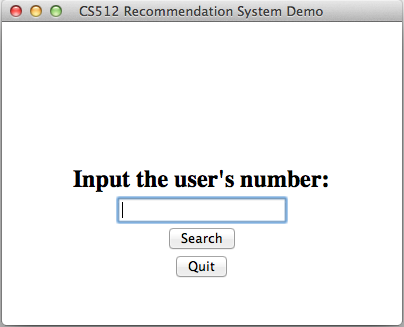
\includegraphics[width=300mm]{UI_Input.png}}}
		\caption{An example of finding the recommendations for user 1}\label{fig:UI_input}
	\end{center}
\end{figure}



\item{}
	The error messages popping-up when users access and/or updates are denied (along with explanations and examples):
	\begin{itemize} 
	\item{The error message: This is an invalid input, please input an integer between 0 to 32133. }
	\item{The error message explanation (upon which violation it takes place):  }
	The error pops up when the input number is out of range, i.e. the input user is not in the database. So the system cannot find such user.
	\item{The error message example according to user(s) scenario(s): Input user number 1000000.}
	\begin{figure}[h] 
	\begin{center}
		\advance\rightskip-1cm
		{\scalebox{0.3}{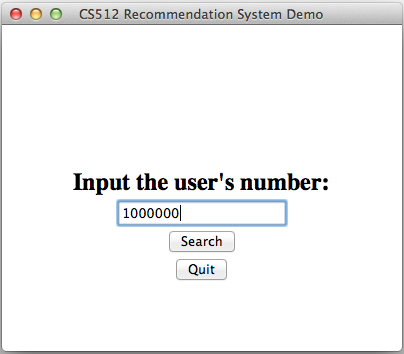
\includegraphics[width=300mm]{UI_Error1.png}}}
	\end{center}
	\end{figure}
	\begin{figure}[h] 
	\begin{center}
		\advance\rightskip-1cm
		{\scalebox{0.3}{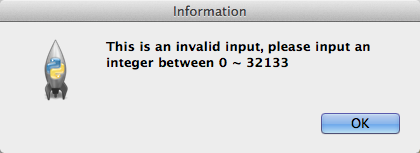
\includegraphics[width=300mm]{UI_Error2.png}}}
		\caption{Error message for inputting invalid user number 1000000}\label{fig:UI_Error}
	\end{center}
	\end{figure}
	
	 \end{itemize}
\item{}
	The information messages or results that pop-up in response to user interface events.
	\begin{itemize} 
	\item{The information message: shown in Fig. 11.}
	\begin{figure}[h] 
	\begin{center}
		\advance\rightskip-1cm
		{\scalebox{0.3}{\includegraphics[width=300mm]{UI_Result.png}}}
		\caption{UI demonstration of resulting recommendation for user 1}\label{fig:UI_Result}
	\end{center}
	\end{figure}
	\item{}
	The recommendation list contains 10 business units that are most likely favorable by input user. 
	 \end{itemize}




\section{Project Highlights.}\label{sec:7. Project Highlights.}

\section{Appendix}\label{sec:Appendix}
\textnormal{
\subsection{Details on edge weight formula in each layers}
\begin{itemize} 
\item{First layer edge weight}
\\$node_edge = RStar$
\\Recall the first layer of our graph is business units that have been reviewed by the input user. The weights on the first layer edges (edges points to first layer) are simply the review of a store by the input user, Users can give review of number from 0 to 5, indicating how much they like the store.
%The SQL tables that represent the ER project model, along with at least 3-5 rows of concrete data per table.
\item{Second layer edge weight}
\\$node_edge = RStar+ RAve()$
\\Recall the second layer of our graph are users who have reviewed a store in the first layer. The weights on the second layer edges are reviews of users in the second layer, adjusted by the average review score for all ratings the particular user previously gave. For example, an edge from layer 1 to 2 indicates how much the store in layer 1 is liked by a user given the user's average review.
%The normalization steps for each table, along with explanations/justifications of each normalization step.
\item{Third layer edge weight}
\\$node_edge = RStar+ RAve()+ Aux(cate,attr)$
\\Recall the elements in the third layer are stores that users in layer two have reviewed. Each of the element in layer three will potentially be in the recommendation list. Here we weigh the third layer edges by adjusted reviews, same as second layer edges, and a auxiliary function which looks into category and attribute of business stores, and further detects similarities between users. For each of the stores in layer 3, we extract it's business category, denoted by A for convenience. Then we calculate the probability that category A appears in layer 1.  Note that the probability represents level of demand in this category by the input user. Suppose the user has a very high demand in category A, we assign this category a higher weight. And on the other hand, if the need is 0, we conclude that the input user does not need recommendation on this kind of service, and we assign a tiny weight to stores in this category, so that it is unlikely to appear in the recommendation list. Attribute factor works in similar way as category.
\end{itemize}
}

%%%%%%%%%%%%%%%%%%%%%%%%%%%%%%%%%%%%%%%%%%%%%%%%%%%%%%%%%%%%%%%%%%%%%%%%%%%%%%%%%%%%%%%%%%%%%%%%%%%%%%%%%%
%\textnormal{
\begin{itemize} 
\item{}
Only working applications will be acceptable at project completion. A running demo shoul be presented to your project advisor at a date to be specified after the second midterm. A version of your application shall be installed in a machine to be specifed later during the semester. Your final submissiom package will also include a final LaTeX report modeled after this document, as well as a Power Point Presentation.
\item{}
The presentation (7 to 8 minutes) should include at least the following items (The order of the slides is important):
\begin{enumerate}
\item{}
Title: Project Names (authors and affiliations)
\item{}
Project Goal
\item{}
Outline of the presentation
\item{}
Description
\item{}
Pictures are essential. Please include Interface snapshots exemplyfing tthe different modes of users's interaction.
\item{}
Project Stumbling Blocks
\item{}
Data collection, Flow Diagram, Integrity Constraints
\item{}
Sample Findings
\item{}
Future Extensions
\item{}
Acknowledgements
\item{}
References and Resources used(libraries, languages, web resources)
\item{}
Demo(3 minutes)
\end{enumerate}
Please follow the sample presentation mock up that is posted on Sakai.
\item{}
By Dec 1 your group should have completed the final submission. This includes a presentation (7 to 8 minutes) to your project advisor as well as a convincing  demo of your project functionalities (3 minutes): every group member should attend the demo (and presentation) indicating clearly  and specifically his/her contribution to the project.  This wil allow us to evaluate all students in a consistent and fair manner.
\item{}
Thank you, and best of luck!
\end{itemize}
}


\bibliographystyle{IEEEtran}
%\bibliography{IEEEabrv,bib_queyroi_abello2013}
%\bibliography{bib_queyroi_abello2013}

\end{document}


